% ============================================================
\section{Introduction}
\label{sec:intro}
% ============================================================

% Restructured 20 Sep 2026 into five paragraphs with one job each, around one running example. The
% previous version opened with the premise and the screen, then a Terminology block, then the
% definition, then contributions -- all true, and a reviewer reported not being able to tell which
% sentence was the one to remember. The Terminology block is gone from here: under the naming
% convention at the end of S3 the body no longer uses bare condition letters, so the block was
% decoding notation the text had stopped using. Everything it defined is still defined in S3.

Fine-tuning a time-series foundation model reshapes its internal
representations, and a large literature treats that reshaping as damage to be
prevented: by freezing the encoder, by regularising toward the pre-trained
weights, by confining updates to low-rank adapters.  Every one of those
prescriptions presupposes that the pre-trained representation was worth
preserving \emph{on the target task}.  \textbf{We test that presupposition on
the benchmarks the field actually uses, and it mostly fails.}

\textbf{One checkpoint, two datasets, opposite lessons.}  Fine-tune Moirai-Base
on ETTh1 and its encoder barely moves (CKA $0.755$ against the pre-trained
encoder), and the model ends $22.8\%$ \emph{worse} than not fine-tuning at all.
Fine-tune the same checkpoint on ETTh2 and the encoder restructures far more, to
CKA $0.460$, and the model ends $31.4\%$ \emph{better}.  Read drift as damage and
you would have protected the run that needed no protection and left alone the one
that did.  The pair is not a curiosity we picked out: within our Moirai-Base cells
the two \emph{least} drifted are the only two that degrade, and the two most
drifted improve the most (\S\ref{sec:exp3}; both pairs are labelled in
Figure~\ref{fig:screen}b).

\textbf{What drift can and cannot tell you.}  CKA tells us that the
representation \emph{changed}.  It takes an intervention (fine-tune the whole
model, then fine-tune it again with the encoder frozen, same data, same epochs) to
tell us whether that change was \emph{valuable}.  \textbf{Across the cells we
evaluate, the former does not reliably predict the latter.}
% Review M7: frame this as falsifying a shortcut in use, not as discovering a principle. Two sentences,
% and the concession that our own earlier draft made the substitution is the strongest form of the point
% -- it is recorded in app:corrections either way, so stating it here costs lines and not credibility.
\textbf{We do not claim that is surprising.}  A post-treatment similarity
statistic has no reason to identify an interventional contrast, and a reader who
finds the negative result obvious is agreeing with us; what we claim is that the
substitution is made anyway (by the prescriptions above, and by an earlier draft
of this work), and that measuring what it costs takes the intervention nobody
runs.  So we split the
practitioner's question into four layers and answer them in order
(Figure~\ref{fig:screen}a): is there a capability
worth preserving at all (\S\ref{sec:forecasting})?  did the representation change
(CKA, \S\ref{sec:exp3})?  did letting the encoder adapt
help or hurt (\S\ref{sec:exp2})?  and does the conjunction of the first and third
amount to destroying a demonstrated capability
(\S\ref{sec:analysis:degradation})?  Layer~2 is the cheap measurement and layer~3
the expensive intervention, so the paper's question is whether the first can stand
in for the second; a fifth section asks whether the whole screen works
\emph{prospectively} (\S\ref{sec:exp4}).

% Figure 1 is declared here rather than at the head of S4 (where it lived until 20 Sep 2026) so that a
% reader meets the paper's one claim, drawn, on page 2 instead of page 5. It is a [t] float and this
% declaration point is past page 1's break, so it cannot be pulled back onto the abstract page. Panel
% (b)'s x-axis is CKA as of this round -- the figure script's docstring records why it was the gate for
% two rounds before that, and the two correlations are printed on the panel either way.
\begin{figure}[t]
\centering
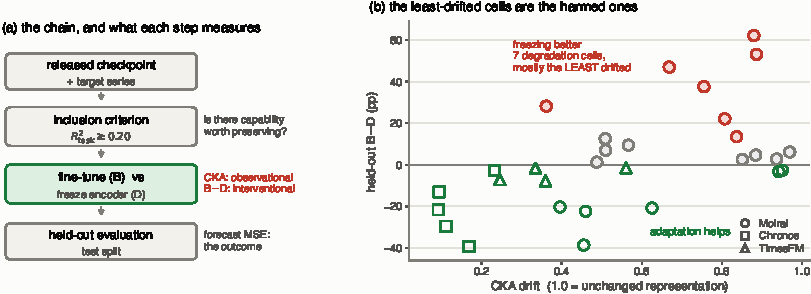
\includegraphics[width=\linewidth]{fig1_diagnostic_flow.pdf}
% Round 7 (C1/C2): the caption was 11 printed lines, and most of them RE-TYPED numbers the panels
% themselves print -- the funnel's boxes and tags carry 7 of 31, "CKA measured on all 31", the 4-of-31
% reversal and the 0-cell verdict; panel (b) prints the best cut's 5 misplacements and both clustered
% rhos in its own text block. Hand-typed copies of computed numbers are exactly the failure mode this
% project keeps hitting, so they are deleted rather than re-verified, and the caption now carries the
% claim, the two things no panel can say (what a filled marker means, what rho is clustered on) and the
% running example. The figure script asserts the Moirai-Base ordering it draws, so the claim below is
% checked at build time and not by a chk() on this caption.
\caption{\textbf{The whole paper}, with every count in both panels computed from
\texttt{cell\_matrix} at build time rather than typed here.  \textbf{(a)}~The four
layers of \S\ref{sec:method} as a funnel over the 31 cells that carry a
selection-split gate: CKA filters none of them, and no cell meets either form of
the degradation definition.  \textbf{(b)}~The same cells as CKA against held-out
$\denc$ (positive ${=}$ freezing better): \textbf{measured drift does not
reliably predict the value of encoder adaptation}, and no cut on CKA separates the
cells adaptation helped from the cells it hurt.  The labelled pairs are the paper's
running example: Moirai-Base's two \emph{least} drifted cells are its only two
that degrade, and its two most drifted improve the most (\S\ref{sec:exp3}).  Filled
markers clear the gate; each $\rho$ is clustered by dataset${\times}$horizon within
Moirai, the only backbone with enough cells to ask
(Appendix~\ref{app:clustered}).}
\label{fig:screen}
\end{figure}

\textbf{Design and scope.}  We screen \textbf{32 cells} across three backbones (Moirai
Small 13.8M, Base 91M, Large 311M; Chronos-T5~\cite{ansari2024chronos};
TimesFM-2.5~\cite{das2024timeseries}, with MOMENT~\cite{goswami2024moment}
screened and excluded), six datasets and two forecast horizons, and pair each with
a full fine-tune and a frozen-encoder run at 3--10 seeds
(\S\ref{sec:forecasting}).  The screen is deliberately weak: it asks only whether
the pre-trained model, zero-shot (ZS), beats a lookback-96 linear regression \emph{fit
on the practitioner's own target data}: not a tuned supervised forecaster, not an
ensemble, a single ridge-OLS map estimated once on the training split and applied
unchanged.  We write that margin against a baseline $b$ as
$\Vb{b} = 1 - \text{MSE}_{\text{ZS}}/\text{MSE}_{b}$ (a \emph{baseline-relative}
advantage, never a property of the checkpoint alone), and score it on windows
disjoint from every outcome we report.  \textbf{Every claim below is about the
checkpoints, datasets and fine-tuning protocols we evaluated}: we do not claim
that fine-tuning is safe, nor that foundation models are useless for forecasting.

\textbf{The result, in three clauses.}  \textbf{Seven of the 31 scored cells}
clear the screen, all of them Moirai and on two of the six datasets: all five of
its ETTh2 cells and two of its four on ETTm2.  Where the advantage does exist,
letting the encoder adapt usually \emph{helps}: full fine-tuning improves MSE on
five of the seven, by 31--42\% on the three ETTh2 cells, and the two whose mean
shows harm carry only 4/10 and 5/10 seeds agreeing on the sign.  And \textbf{no
cell shows decisive evidence of harm}: on multiplicity-adjusted paired intervals
only 2 of the 31 favour freezing, and both are cells the screen
\emph{rejects} (\S\ref{sec:analysis:degradation}).

\textbf{Contributions.}

\begin{enumerate}\itemsep1pt
  \item \textbf{A negative result on the premise of forgetting mitigation.}
    Screened against a linear regression fit on the target data, only 7 of 31
    cells show a pre-trained advantage to preserve, and all seven are Moirai,
    five on ETTh2 and two on ETTm2; four of the seven are \emph{improved} by full
    fine-tuning in every seed, three of them by 31--42\% (\S\ref{sec:forecasting}).

  \item \textbf{The intervention contrast as the estimand, and drift as a failed
    predictor of it.}  We name $\denc$ (full fine-tuning minus a frozen
    encoder) as the quantity this design manipulates, and show that CKA
    \textbf{does not provide a reliable ordering} of it across an outcome spanning
    $-51.8\%$ to $+46.1\%$: within-backbone $\rho{=}{+}0.168$ with clustered CI
    $[-0.469,{+}0.717]$ \emph{within Moirai}, the only backbone with enough cells to
    ask, with Chronos and TimesFM read qualitatively beside it rather than pooled
    with it, and with no actionable threshold anywhere (\S\ref{sec:exp3}).

  \item \textbf{No cell shows decisive evidence of harmful encoder adaptation}
    (2 freezing-better, 4 adaptation-better, 25 inconclusive at a
    multiplicity-adjusted $q{<}0.05$; zero under the pre-registered unanimity
    criterion), so the value gate we proposed has no positive instance to
    predict: TP~0, FP~8 on
    eight cells whose predictions were frozen in git before those cells were
    trained, and $\rho{=}{-}0.293$ against the intervention outcome within
    Moirai; a direction, not an interval claim (\S\ref{sec:exp4}).  A
    reproducibility bundle (configs, seed lists, metric scripts, uni2ts patch,
    both linear baselines) accompanies this paper.
\end{enumerate}

% "Those four" was correct until this round's contribution item 3 -- the third statement of the two
% boxed lessons -- was cut. The list is three items now, so the count is corrected here rather than the
% cut reverted: nothing was withdrawn, the lessons are stated in the abstract and in S3's box.
\textbf{What is a claim here, and what is a control.}  Those three are the paper's
claims, argued in \S\S\ref{sec:forecasting}--\ref{sec:exp4}.  Everything else is a
control or a boundary case, labelled where it appears: influenza-like illness
(ILI) and an IoT anomaly detector are external cells that gate-fail, reported as case
studies rather than evidence (Appendix~\ref{app:ili_gate}); the mitigation spectrum,
strict freeze and the LoRA sweeps ask only whether the frozen-encoder comparison
depends on how it is implemented
(Appendices~\ref{app:full_tables},~\ref{app:strictfreeze},~\ref{app:lora_rank}).
No claim above rests on any of them.
% The retraction pointer that stood here is cut for page room, not withdrawn: S8 item (5) states that
% the probe axis is retracted and points at the same appendix, and S9's Research Integrity statement
% and Appendix app:corrections carry the full record. Cutting the restatement, not the record.
